\section{Results and discussions}

Many different simulations were run and captured in video form. All the useful videos recorded can be found \href{https://drive.google.com/drive/folders/1YSsqFpuCf-zBKHXfOGs2zDYO57xDAOi-?usp=sharing}{here}. \\

The simulations were ran with gaussian disturbances being added in every timestep. Hence, two different runs of the same simulation would yield different results. On an average, the results are acceptable, but there are still times when the fuzzy controller isn't able to stabilize the system for higher disturbance levels. \\

Having given that disclaimer, results from one run of the PID and FLC simulations are shown below, in figs. \ref{fig:PID} and \ref{fig:FLC} respectively. 

\begin{figure}[h!]
    \centering
    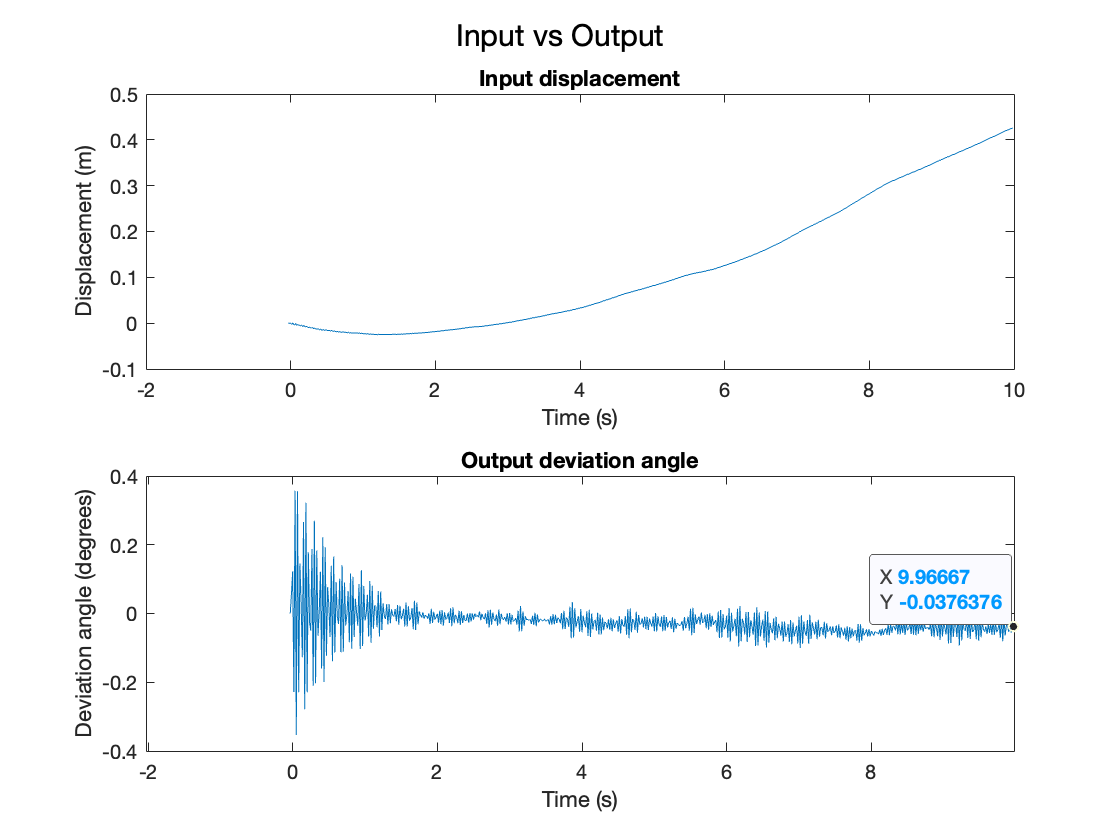
\includegraphics[scale=0.35]{images/PID.png}
    \caption{ PID controller output }
    \label{fig:PID}
\end{figure}

\pagebreak

\begin{figure}[h!]
    \centering
    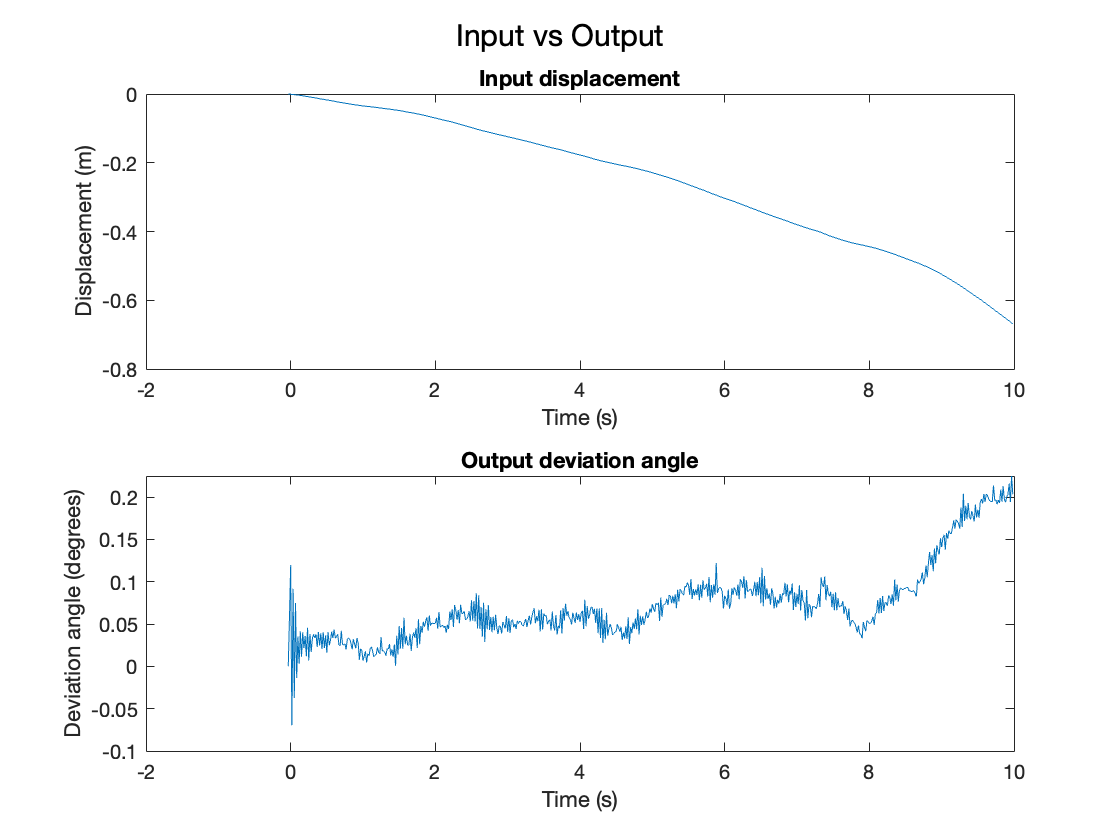
\includegraphics[scale=0.35]{images/FLC.png}
    \caption{ FLC output }
    \label{fig:FLC}
\end{figure}

It is to be noted that with disturbances, both controllers often struggle to bring the pendulum back to the zero position. However, both controllers are able to stabilize the system with reasonable degree of success, though not nearly sufficient for industrial use.

